\title{Math 239 Fall 2023 Tutorial Answers Week 10}

\date{2023 Nov. 23/24}
\maketitle

\begin{enumerate}
    \question{Planarity and Graph Complements} 
    \begin{enumerate}
        \item There are numerous solutions. Here are some examples.
        \begin{figure}[hbt!]
            \centering
            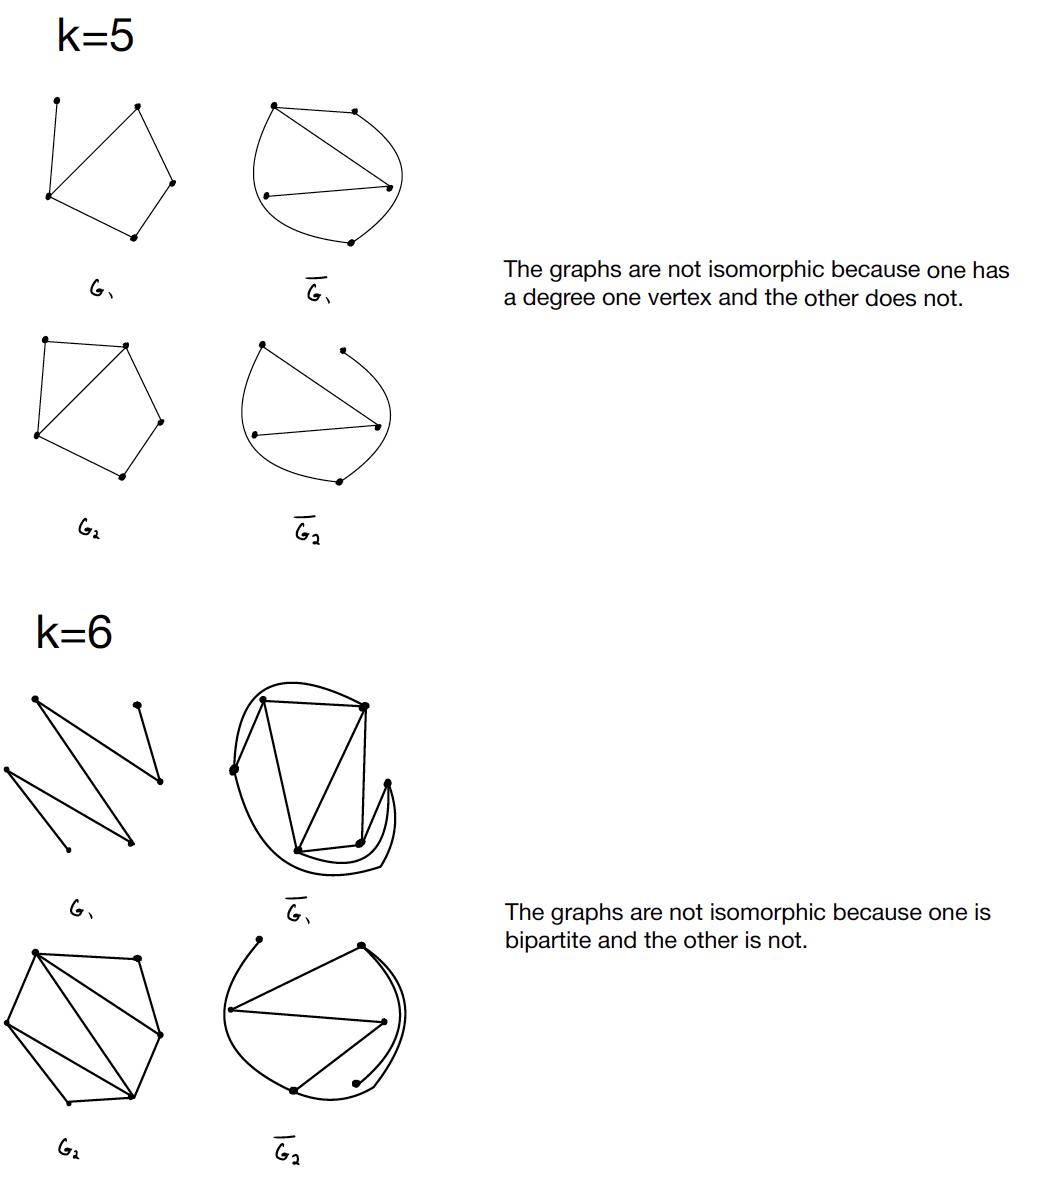
\includegraphics[scale=.6]{Screenshot 2023-11-20 at 5.03.50 PM.png}
        \end{figure}
        \item Let $G$ be $K_{3,3}$ plus five isolated vertices. 
    \end{enumerate}


   
    \question{Cartesian Product of Graphs} 
    \begin{enumerate}
    \item Let $(a_1, b_1)(a_2, b_2) \in E(G \square H).$ That is, by definition, either $a_1 = a_2$ and $b_1b_2 \in E(H)$, or $a_1a_2\in E(G)$ and $b_1 = b_2$. Suppose the former. Then $\phi_1(a_1) = \phi_1(a_2)$ since $a_1 = a_2$. On the other hand $\phi_2(b_1) \neq \phi_2(b_2)$ since $b_1b_2 \in E(H)$ and $\phi_2$ is a $k$-coloring of $H$. Thus, since $\phi_2$ assigns colors $\{1,\cdots,k\}$, we find that 
    \[\phi_2(b_1) \neq \phi_2(b_2) \mod{k}.\]
It follows that 
\[\phi((a_1, b_1)) = \phi_1(a_1) + \phi_2(b_1) \mod{k} \neq \phi_1(a_2) + \phi_2(b_2) \mod{k} = \phi((a_2, b_2)).\]
    [Note one could just say what is written below follows by symmetry, but we include it
for completeness]
So we assume the latter case. Then $\phi_2(b_1) = \phi_2(b_2)$ since $b_1 = b_2$. On the other hand, $\phi_1(a_1) \neq \phi_1(a_2)$ since $a_1a_2 \in E(G)$ and $\phi_1$ is a $k$-coloring of $G$. Thus, since $\phi_1$ assigns colors $\{1,\cdots,k\},$ we find that 
\[\phi_1(a_1) \neq \phi_1(a_2) \mod{k}\]
It follows that
\[\phi((a_1,b_1)) = \phi_1(a_1) + \phi_2(b_1) \mod{k} \neq \phi_1(a_2) + \phi_2(b_2) \mod{k} = \phi((a_2, b_2)).\]
Hence $\phi$ is a $k$-coloring of $G\square H$ as desired.
\item Let $k=\max\{k_1,k_2\}.$ Since $G$ is $k_1$-colorable, $G$ has a $k_1$-coloring $\phi_1$. Since $k \geq k_1$, we have that $\phi_1$ is also a $k$-coloring of $G$. Similarly, since $H$ is $k_2$-colorable, $H$ has a $k_2$-coloring $\phi_2$. Since $k \geq k_2$, we have that $\phi_2$ is also a $k$-coloring of $H$.

Let $\phi$ be as defined in part (a). By part (a), $\phi$ is a $k$-coloring of $G\square H$. Hence $G\square H$ is $k$-colorable as desired.
\end{enumerate}
    \question{Graph Coloring} We will prove this by induction on the number of vertices, $n$.

    \textbf{Base Case:} $n = 1$. $G$ is a single vertex, which is $k+1$-colorable. 
    \textbf{Induction Hypothesis:} Assume every graph on $n-1$ vertices where every non-empty subgraph contains a vertex of degree at most $k$ is $(k+1)$-colorable.

    \textbf{Inductive Step:} Let $G$ be such a graph with $n$ vertices. Let $v$ be a vertex of degree at most $k$ (it must exist, as $G$ is a subgraph of itself). Let $G' = G - v$. Since $G'$ is a subgraph of $G$, it also contains a vertex of degree at most $k$. By the induction hypothesis, $G'$ is $(k+1)$-colorable. We can extend this to a coloring of $G$ by coloring $v$ with a color that isn't used by any of its neighbors, which much exist since $v$ has at most $k$ neighbors and we have $k +1$ colors to choose from. 

    Graphs that satisfy the description that are not $k$-colorable include $K_n$ and odd cycles. 

   
    \question{A Second Planarity Question}
    \begin{enumerate}
        \item This is non-planar with a $K_{3,3}$ edge subdivision.
        \begin{center}
        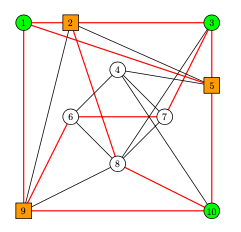
\includegraphics[scale=0.5]{t10q4sol1.png}
        \end{center}
        \item This is planar with the following planar embedding.
        \begin{center}
        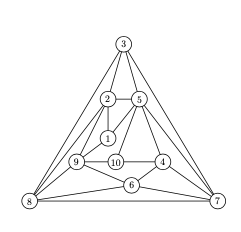
\includegraphics[scale=0.5]{t10q4sol2.png}
        \end{center}
        \item This is planar with the following planar embedding. This is an important example! An edge subdivision CANNOT use one of the vertices in two edges.
        \begin{center}
        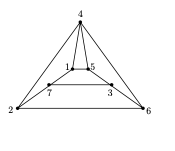
\includegraphics[scale=0.5]{t10q4sol3.png}
        \end{center}
    \end{enumerate}
\end{enumerate}